\documentclass[12pt]{article}
\usepackage[left=1in,top=1in,right=1in,bottom=1in]{geometry}
\usepackage[font=footnotesize]{caption}
\usepackage{parskip}
\usepackage{times}
\usepackage{graphicx}
\usepackage{mathtools}
\usepackage{gensymb}
\usepackage{placeins}
\usepackage{graphicx}
\usepackage{enumitem}
\usepackage{verbatim}	% code text
\usepackage{siunitx}	% math units
\usepackage{hyperref}	% include urls

\setlength{\parskip}{\baselineskip}
\setlist[itemize]{noitemsep}
\setlist[enumerate]{noitemsep}

\begin{document}

	\section{Coordinate System}
	
	We usually represent the angular orientation of an aircraft using Tait-Bryan Angles following \\
	$z$-$y'$-$x''$ (intrinsic rotations) convention, also known as nautical angles, 
	also known as heading, elevation and bank, also known as yaw, pitch and roll. 
	The latter three terms are also used for the three aircraft principal axes.
	
	Some terminology:
	\begin{itemize}
		\item Let $x_b$ be the longitudinal axis (roll), out the nose of the plane.
		\item Let $y_b$ be the lateral axis (pitch), out the right wing.
		\item Let $z_b$ be the vertical axis (yaw), pointing out the bottom of the plane.
	\end{itemize}
	
	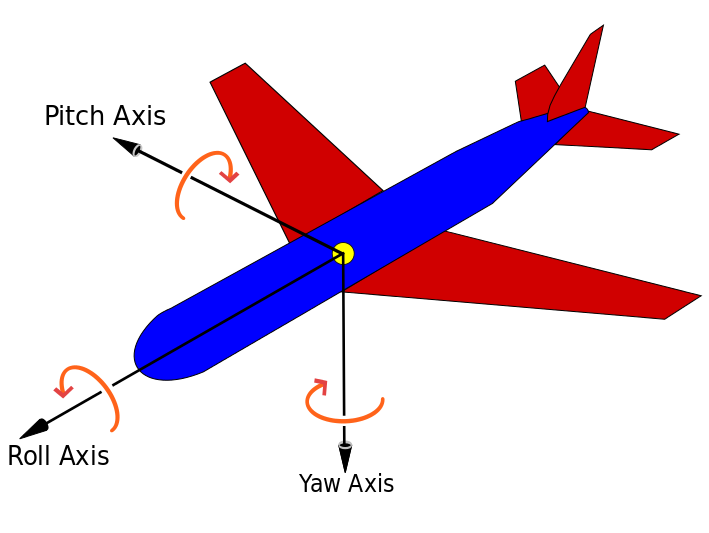
\includegraphics[width=4in]{aircraft_axes.png}
	
	By default, this coordinate system is aligned with the Earth frame:
	\begin{itemize}
		\item $x_b = x_E$ - positive in the direction of north
		\item $y_b = y_E$ - positive in the direction of east
		\item $z_b = z_E$ - positive towards the center of the Earth
	\end{itemize}
	
	To define an arbitrary angular orientation, we follow this procedure:
	\begin{enumerate}
		\item Yaw by $\psi$ about $z_b$.
		\item Pitch by $\theta$ about $y_b$.
		\item Roll by $\phi$ about $x_b$.
	\end{enumerate}
	Note that the body frame rotates with the aircraft as we go through the procedure. 
	Note also that right hand rule convention is always followed.
	
	Note that this can be equivalently represented with the $z$-$y$-$x$ (extrinsic rotations) convention:
	\begin{enumerate}
		\item Roll by $\phi$ about $x_E$.		
		\item Pitch by $\theta$ about $y_E$.
		\item Yaw by $\psi$ about $z_E$.		
	\end{enumerate}
	
	\section{Controller}
	
	We want to control the pitch and roll of the aircraft. 
	(We've given up on yaw because using gravity with the Launchpad only gives us about two detectable axes of rotation.)
	
	More specifically, we want to map the angular position of the joystick to
	an angular position for the elevators and ailerons in the flightsim physics calculations. 
	Let $\vec{g}$ be the acceleration of gravity in the coordinate system of the control column.
	Then define the following functions:
	\begin{itemize}
		\item $\text{jpitch} : \vec{g} \mapsto \theta$
		\item $\text{jroll} : \vec{g} \mapsto \phi$
	\end{itemize}
	
	\section{Method: Simple projection}
	
	We want the position of the controller to correspond the position of the elevators and ailerons.
	i.e., if we pitch the controller forwards, we expect the aircraft to do the same. 
	
	We will define three mutually orthogonal axes in the reference frame of the controller with the following unit vectors:
	\begin{itemize}
		\item $\vec{s}$ (\verb|STICK|) : The direction of the grippy part of the joystick if this were a normal joystick. Points away from the centre of the earth when controller is in rest state.
		\item $\vec{p}$ (\verb|PITCH_AXIS|) : The rotation axis for pitch. Points right when controller is in rest state.
		\item $\vec{r}$ (\verb|ROLL_AXIS|) : The rotation axis for roll. Points forward when controller is in rest state.
	\end{itemize}
	
	The Launchpad will detect an acceleration vector $\vec{g}$ that is pointing out from the centre of the Earth. 
	Assuming that other accelerations such as those from moving the controller are negligible, we now have a vertical reference. 
	
	Assume the following:
	\begin{itemize}
		\item If $\vec{g} \parallel \verb|STICK|$, then $\theta = \phi = \SI{0}{\radian}$
		\item For pitching, consider only the projection of $\vec{g}$ in the $\langle \vec{s}, \vec{r} \rangle$-plane.
		\item For rolling, consider only the projection of $\vec{g}$ in the $\langle \vec{s}, \vec{p} \rangle$-plane.
	\end{itemize}
	
	\textbf{Joystick Pitch}
	
	Here, $\theta$ increases as you tilt the joystick back
	and $\theta$ decreases as you tilt the joystick forwards.
	That is, the sign of the angular displacement is as you would expect
	from a right hand rule rotation of the joystick about $\vec{p}$.	
	\begin{center}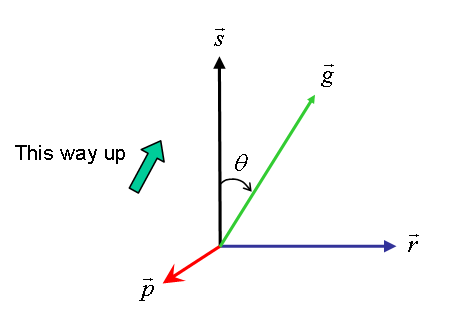
\includegraphics{jpitch.png}\end{center}
	However, keep in mind that in the joystick reference frame,
	$\vec{g}$ will appear to rotate clockwise about $\vec{p}$ as $\theta$ increases,
	opposite of right hand rule. From trig,
		$$\theta = \text{atan2}(\vec{g} \cdot \vec{r}, \vec{g} \cdot \vec{s})$$	
	\textbf{Joystick Roll}
	
	Here, $\phi$ increases as you tilt the joystick right
	and $\phi$ decreases as you tilt the joystick left.
	That is, the sign of the angular displacement is as you would expect
	from a right hand rule rotation of the joystick about $\vec{r}$.
	\begin{center}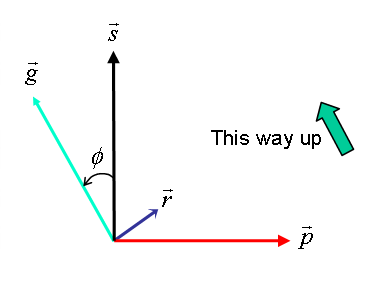
\includegraphics{jroll.png}\end{center}
	However, keep in mind that in the joystick reference frame,
	$\vec{g}$ will appear to rotate clockwise about $\vec{r}$ as 
	$\phi$ increases, opposite of right hand rule. From trig,
		$$\phi = \text{atan2}(-\vec{g} \cdot \vec{p}, \vec{g} \cdot \vec{s})$$

	We can cap $\theta$ and $\phi$ at $\tfrac{\pi}{2}$ and $\tfrac{-\pi}{2}$ to avoid excessive angles.
	
	\subsection{Limitations}
	
	Consider the case where we roll the controller left more than 90$\si{\degree}$. 
	The above formulas will suddenly output maximum pitch, which is not an intuitive response.
	This happens because as soon as we roll left more than 90$\si{\degree}$, the projection of $\vec{g}$ onto the $\langle \vec{s}, \vec{p}_\perp \rangle$-plane suddenly jumps from point up to pointing down,
	which is the same as a sudden jump from 0$\si{\degree}$ to 180$\si{\degree}$.
	
	In normal operation, the user shouldn't really tilt the controller more than 90$\si{\degree}$ from the vertical, so hopefully this won't really matter.
		
	\section{References}

	\urlstyle{same}
	
	\begin{itemize}
		\item Tait-Bryan angles: \url{https://en.wikipedia.org/wiki/Euler_angles#Tait.E2.80.93Bryan_angles}	
		\item Degrees of freedom (mechanics): \url{https://en.wikipedia.org/wiki/Degrees_of_freedom_(mechanics)}
		\item Orientation, Rotation, Velocity and Acceleration,
and the SRM: \url{http://www.sedris.org/wg8home/Documents/WG80485.pdf}
	\end{itemize}

\end{document}